\section{Experiments \& Results}

The experiments were run in two Parts; Part 1- A classification task to classify a dataset containing 3 classes and 
Part 2- A classification task to classify the `MNIST' dataset.

\begin{figure}
    \centering
    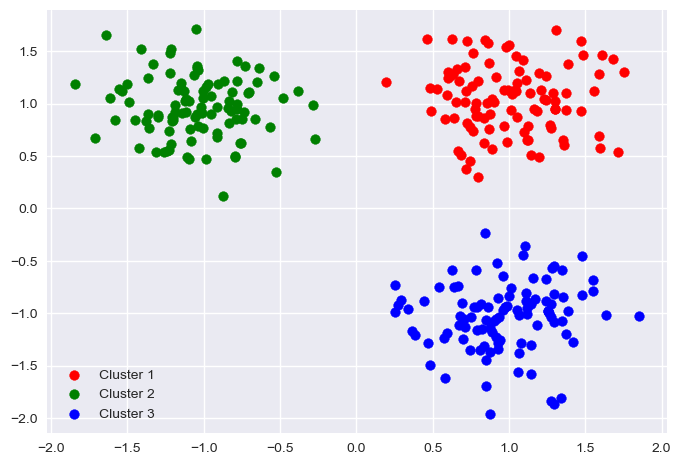
\includegraphics[width=0.5\textwidth]{part_1_data.png}
    \caption[short]{Synthetic data}
    \label{fig: Synthetic data}
\end{figure}

\subsection{Training details}


\subsection{Part 1}

In this portion of the report, we delve into the experiments conducted and the
corresponding results obtained. Our primary objective was to ascertain the 
functionality of the developed program. A secondary goal involved investigating 
the effects of various activation functions: \textbf{Rectified Linear Unit (ReLU)}, 
\textbf{Sigmoid}, and \textbf{Hyperbolic Tangent (Tanh)} and the optimizers: 
\textbf{Stochastic Gradient Descent} and \textbf{Adaptive Momentum (Adam)}. 

\subsubsection{Data}
The dataset utilized for 
this analysis, depicted in Figure \ref{fig: Synthetic data}, was specifically 
crafted to be linearly separable. This design choice was made to simplify the 
verification process, as creating a discriminant function for a linearly 
separable dataset is relatively straightforward for a Neural Network employing 
non-linear activation functions. To this end, multiple architectures were 
explored, each incorporating one of the three aforementioned activation 
functions across all hidden layers. This approach facilitated a comparative 
analysis of the activation functions' performance within the framework of 
Multi-Layer Perceptron (MLP) models. 

\subsubsection{Model Architectures}
The `base model' was a 1 layered model shown in figure \ref{fig: NN 1l} that 
used the sigmoid activation function across its hidden layers, . This architecture was 
designed with the minimum number of neurons required to create 3 functions in the
hidden layer which were supposed to have separated the 3 classes.

3 more `2 (hidden) layered models' (figure \ref{fig: NN 2l}) were created to compare firstly, the activation
functions and secondly, to compare 2 layered models to the base 1 layered model.


\begin{figure}
    \centering
    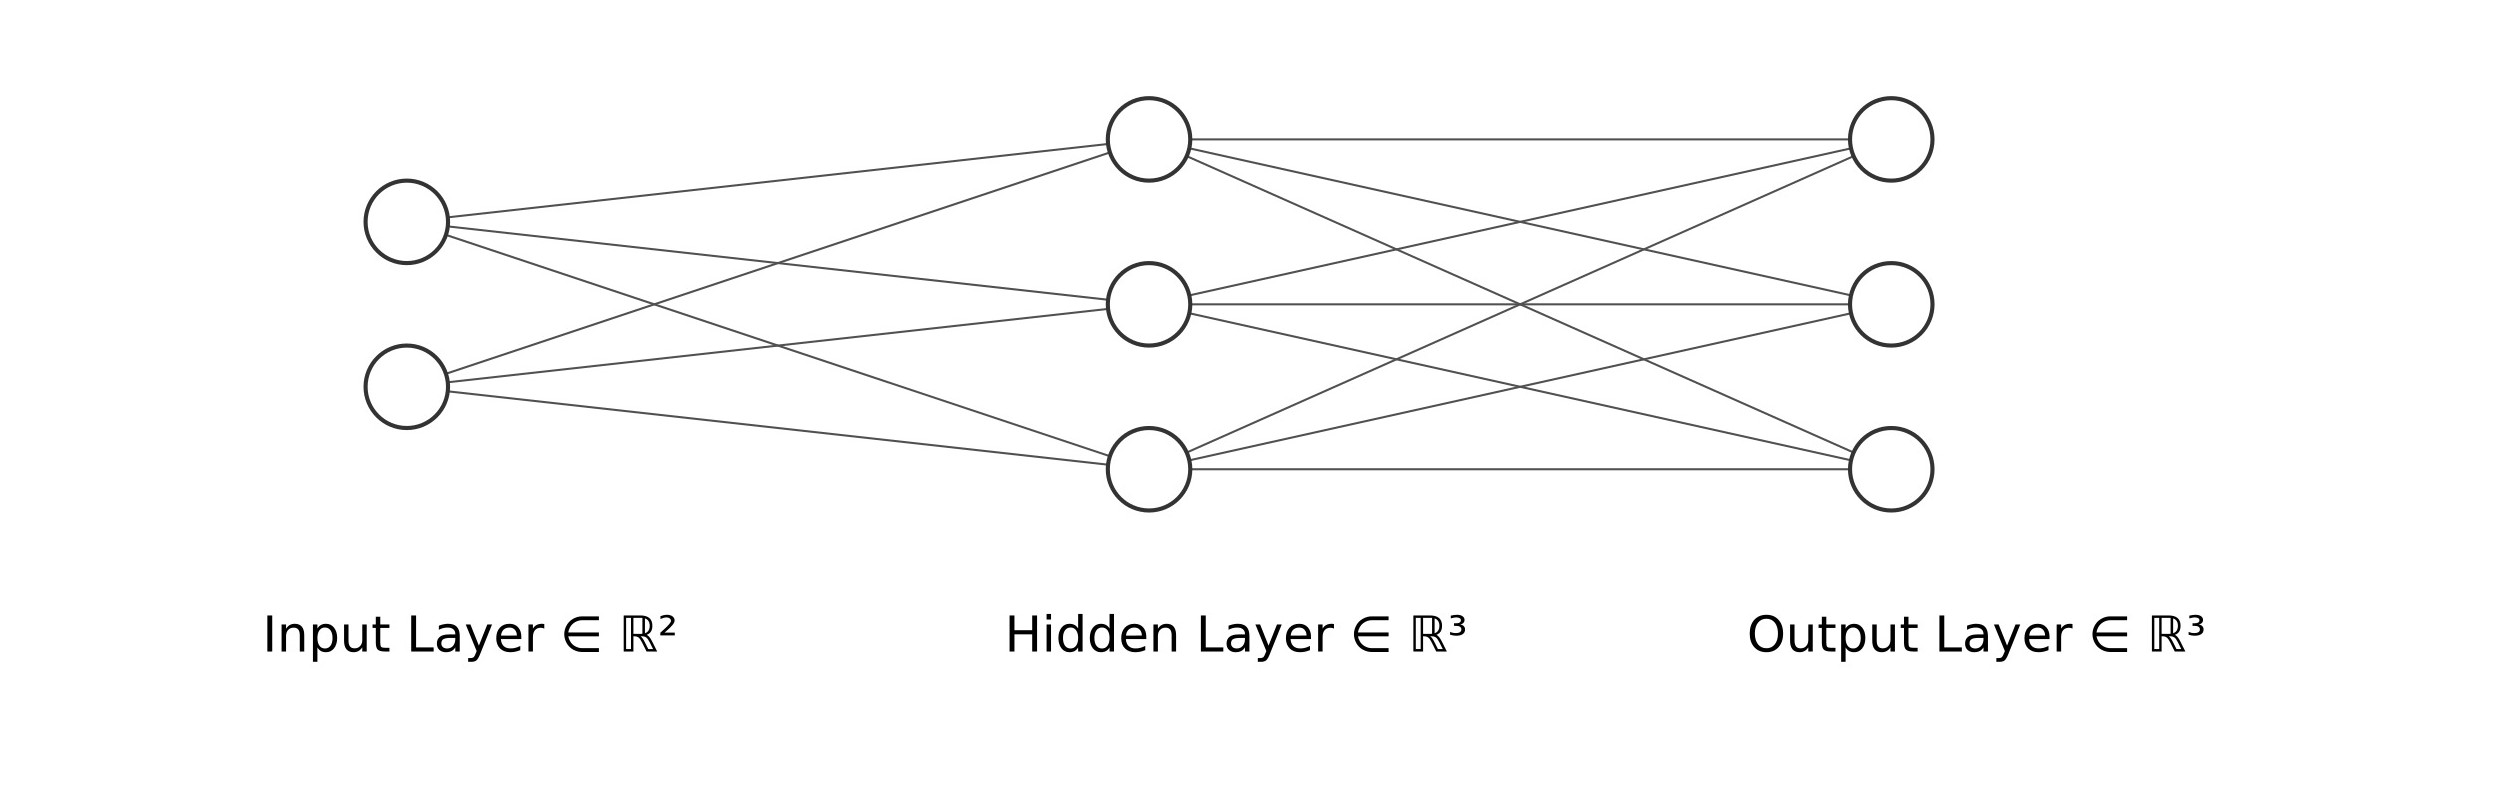
\includegraphics[width=0.8\textwidth]{sigmoid_1_layer.jpg}
    \caption{MLP with 1 hidden layer}
    \label{fig: NN 1l}
\end{figure}

\begin{figure}
    \centering
    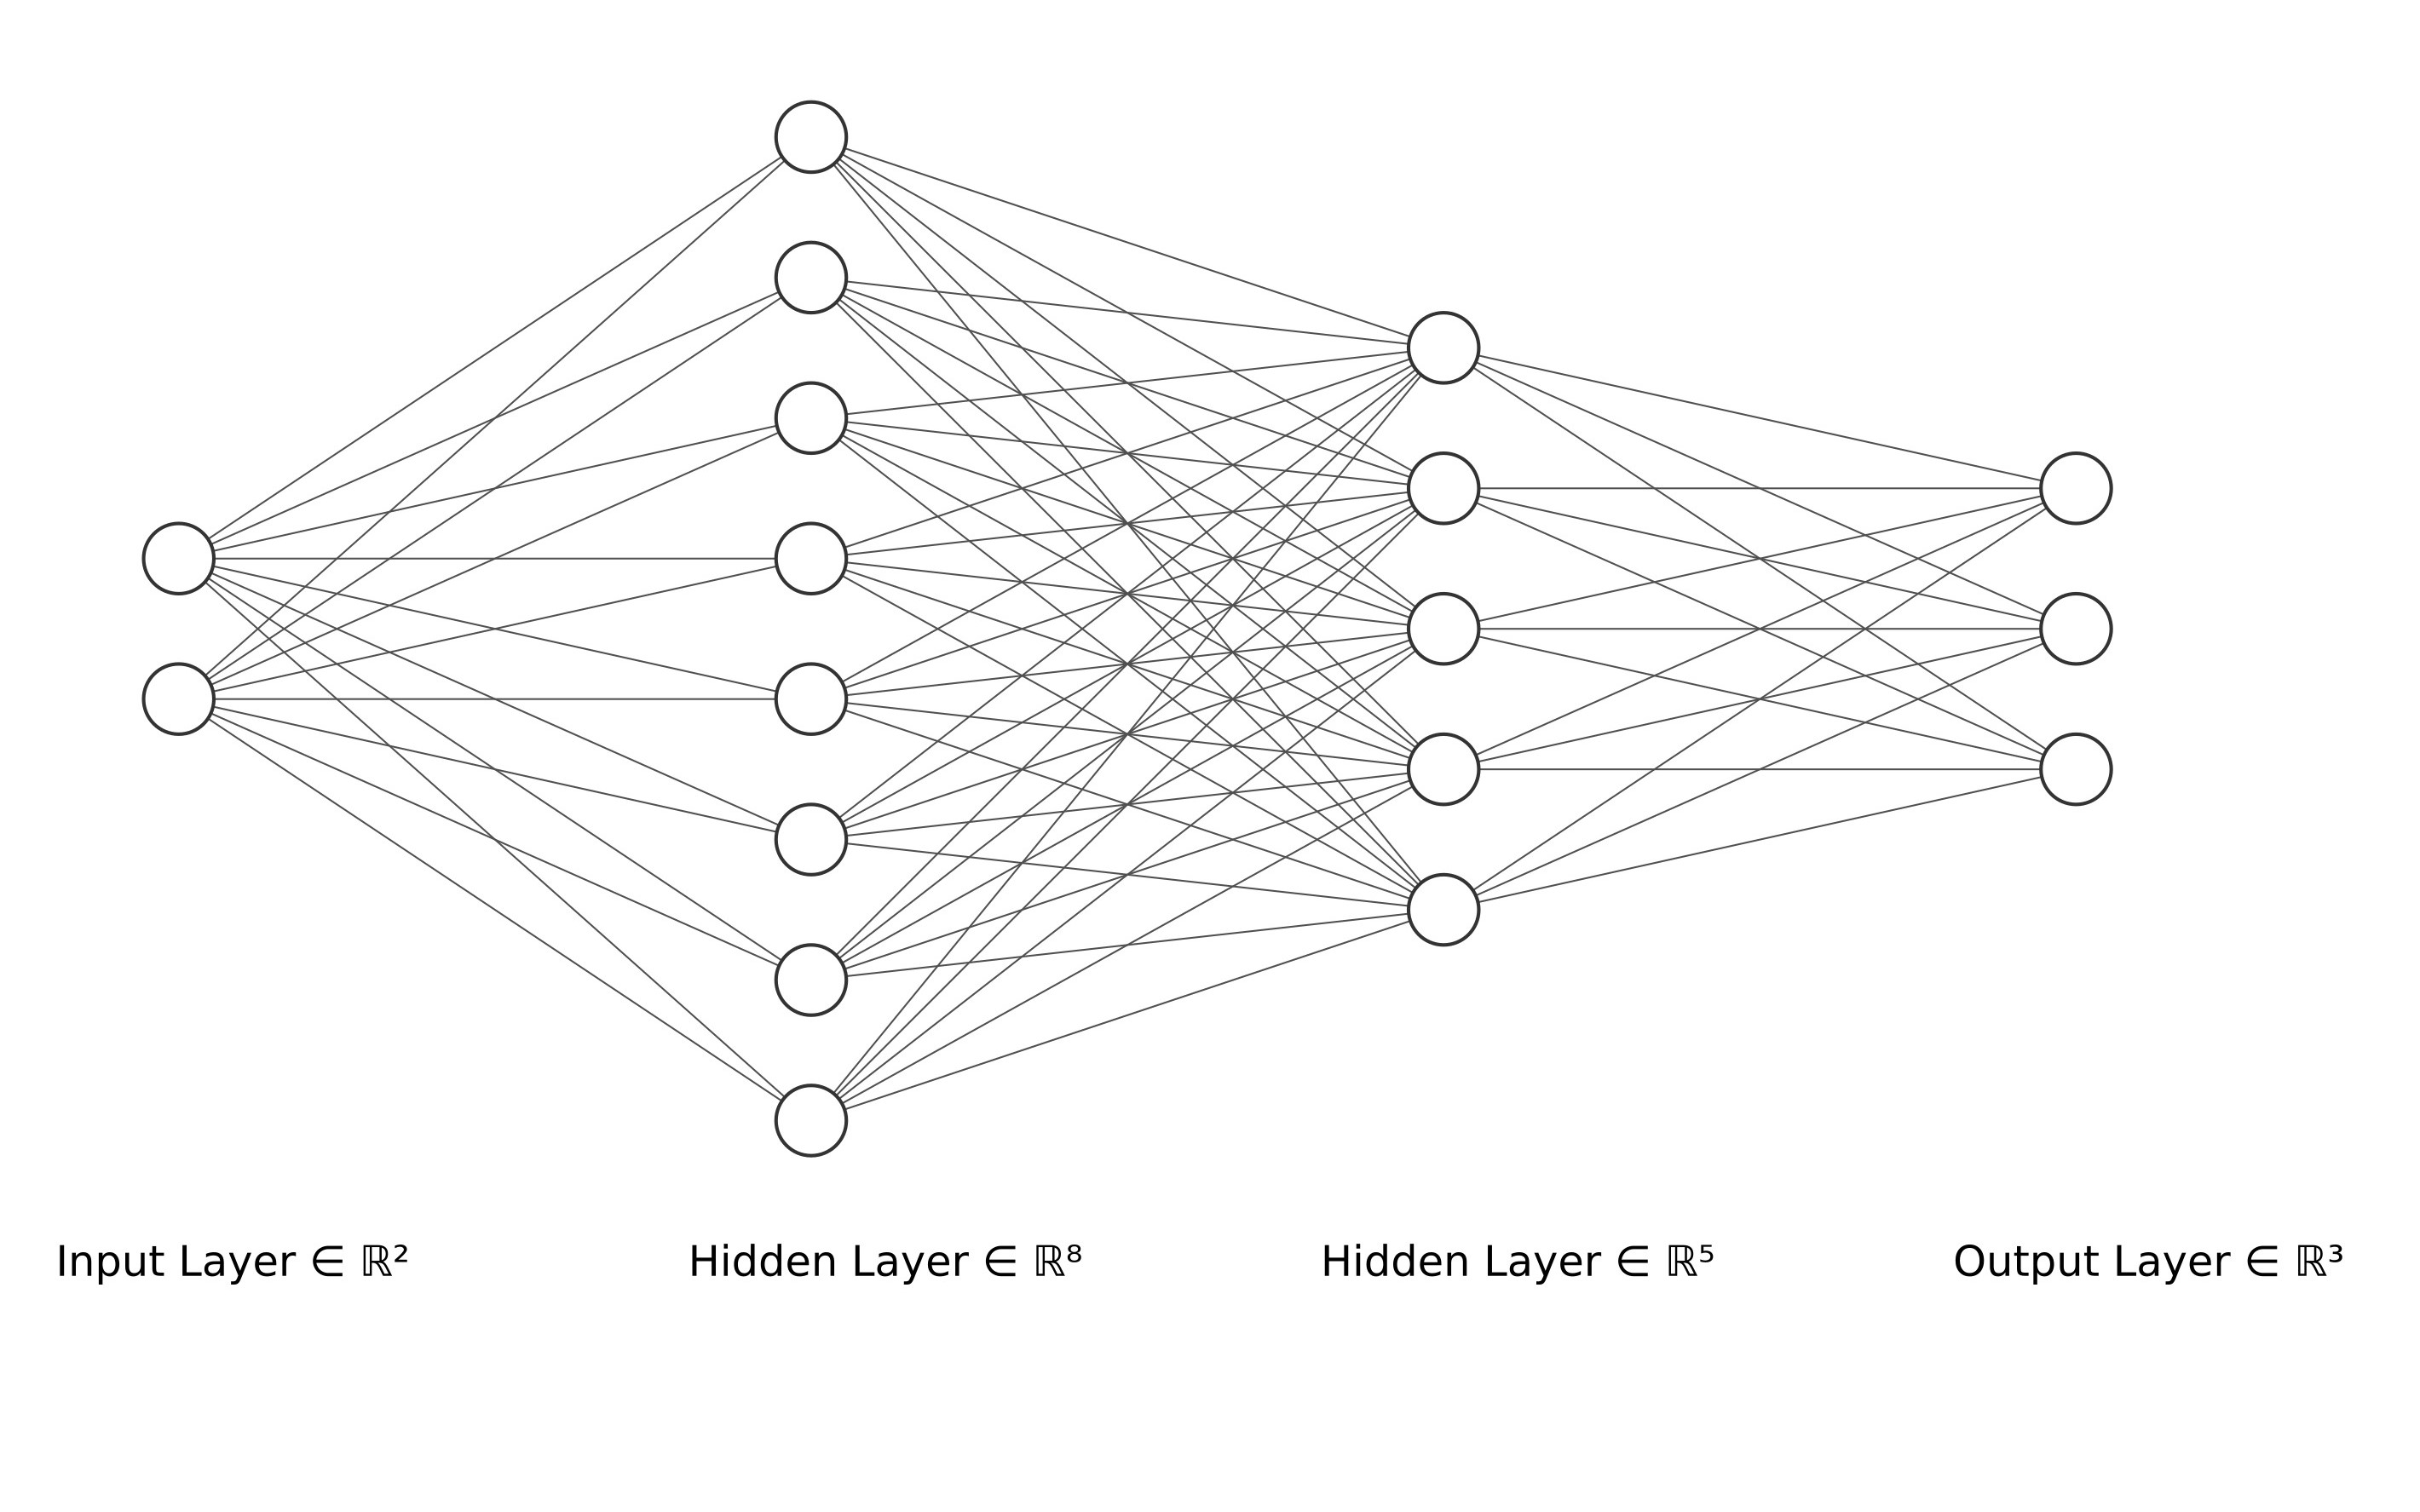
\includegraphics[width=0.8\textwidth]{sigmoid_2_layers.jpg}
    \caption{MLP with 2 hidden layers}
    \label{fig: NN 2l}
\end{figure}


\subsubsection{Results}

The epoch-accuracy (validation set) plots for all the architectures are shown in figure 
\ref{fig: Accuracy}. The epoch-loss plots for the training and validation sets are shown in figure \ref*{fig: loss curves-Adam}
and figure \ref{fig: loss curves-SGD}. The adam optimizer was able to optimize
all models such that they achieved near 100\% accuracy whereas SGD was only able
to optimize the models with 2 layers using the Hyperbolic Tangent and the Rectilinear
Unit function. The Adam optimizer optimized the models faster. If compared on the 
two models where the SGD achieved near 100\% accuracy, the Adam optimizer optimized 
the Tanh model in 5 epochs and the ReLu model in 12 epochs where as the SGD took 
close to a 100 epochs for the ReLu model and about 55 epochs for the Tanh model.
Remarkably, the 1 layered sigmoid model spiked in accuracy at the 62nd epoch and 
started decreasing (and kept decreasing until the end of the experiment) at the 
70th epoch. During these times (62nd to 70th epoch), the average loss over all a batch never changed
for this model. In fact, the loss never changed throughout training. 

The confusion matrices in figure \ref*{fig: cm SGD} indicate that the sigmoid model with
1 hidden layer classified every datapoint as class 1 whereas the one with 2 hidden 
layers classified all datapoints belonging to class - 2 as class - 0. The confusion matrix in
figure \ref*{fig: cm adam} represents the conclusion matrix for architectures, but 
optimized with the adam optimizer.


\begin{figure}
    \centering
    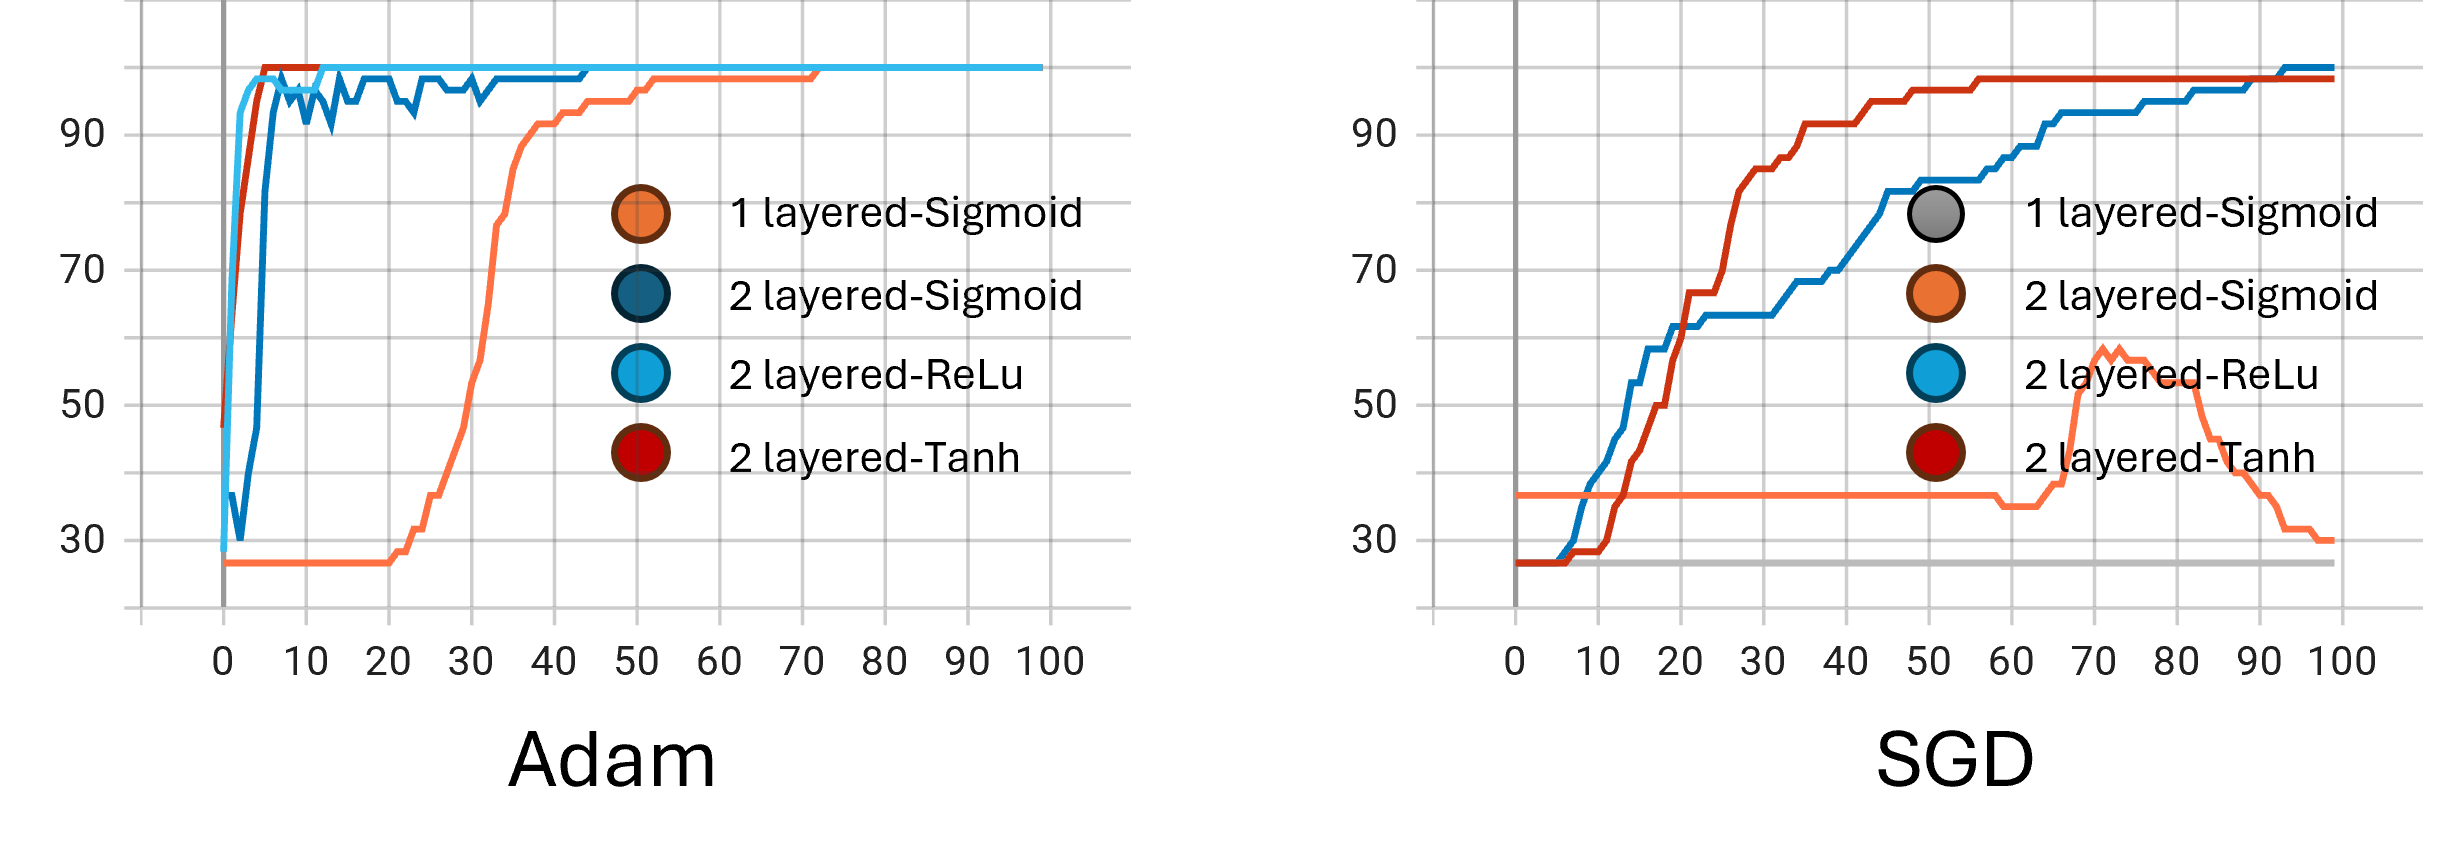
\includegraphics[width=1.0\textwidth]{./results/part_1/accuracy.png}
    \caption{Accuracy on validation set}
    \label{fig: Accuracy}
\end{figure}

\begin{figure}
    \centering
    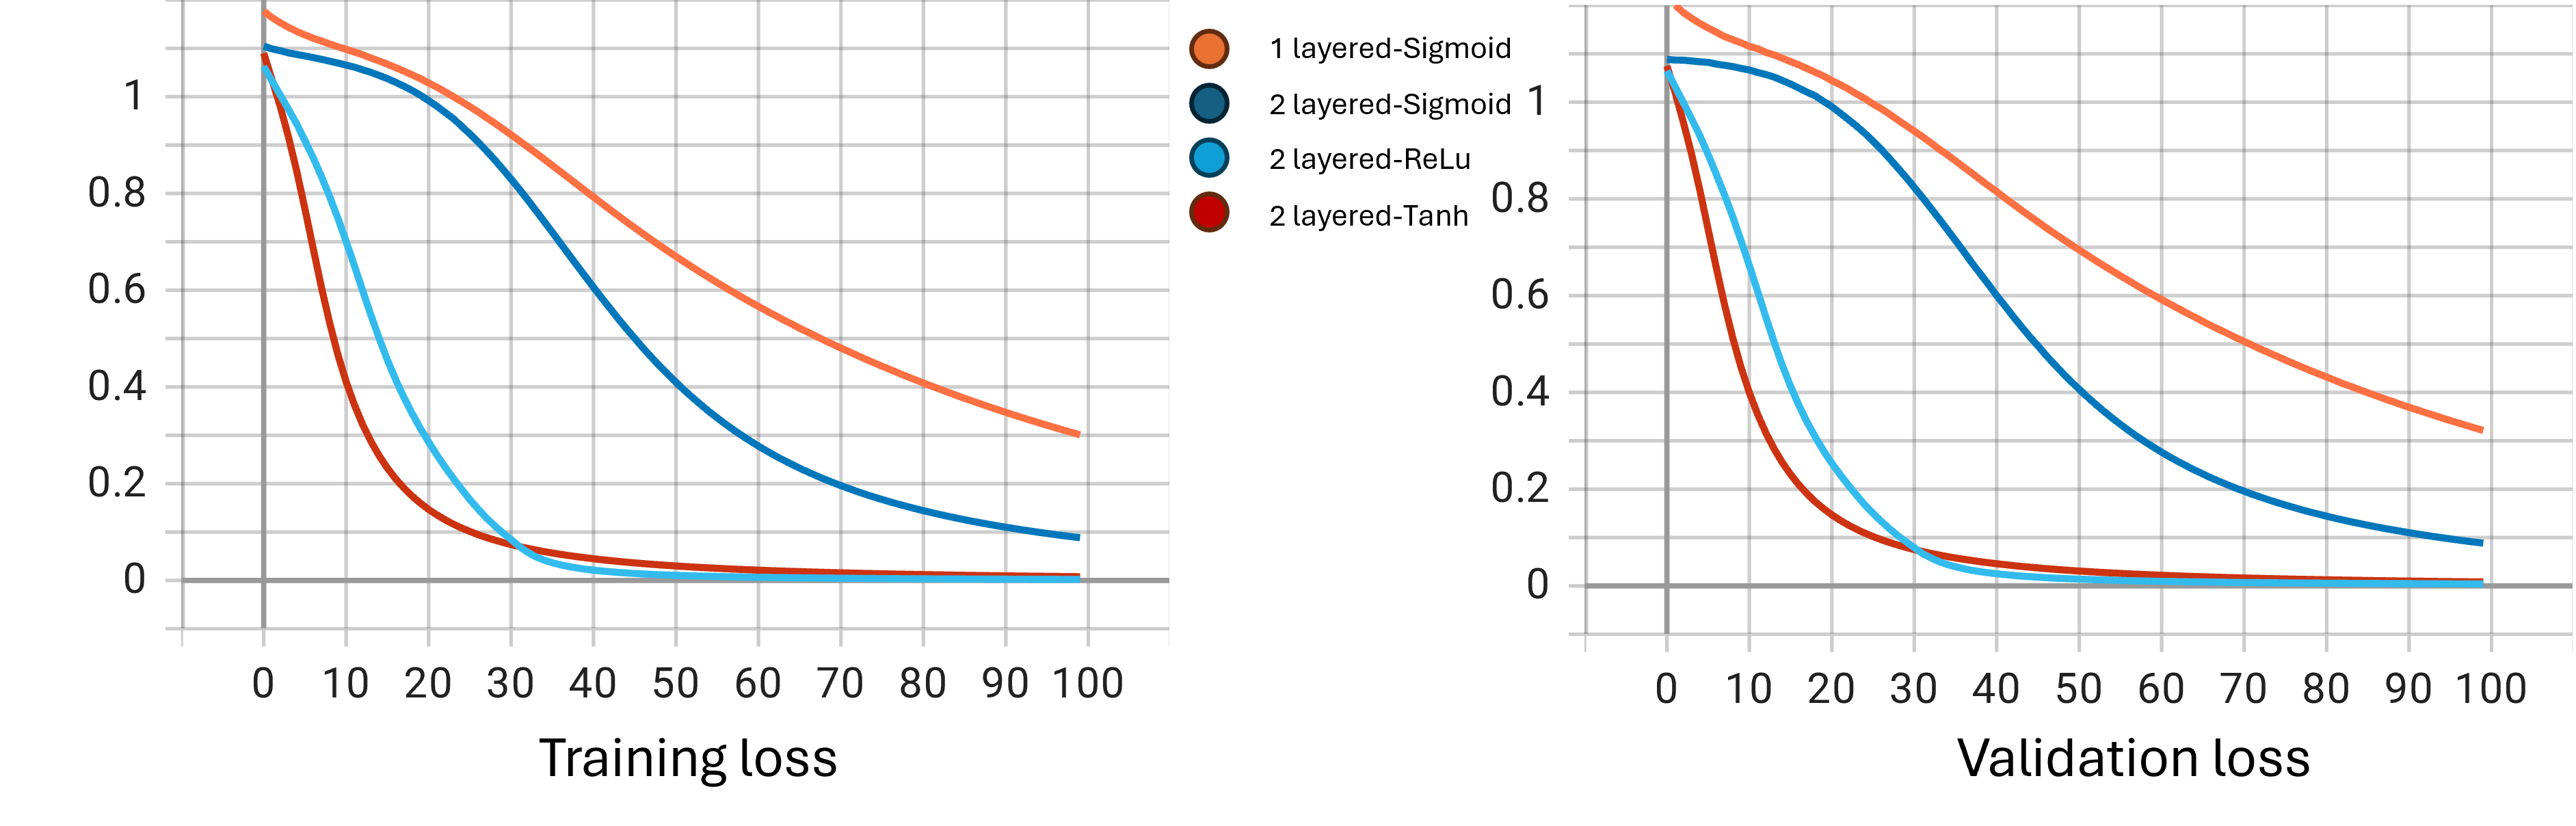
\includegraphics[width=1.0\textwidth]{./results/part_1/loss_adam.png}
    \caption{loss Adam}
    \label{fig: loss curves-Adam}
\end{figure}

\begin{figure}
    \centering
    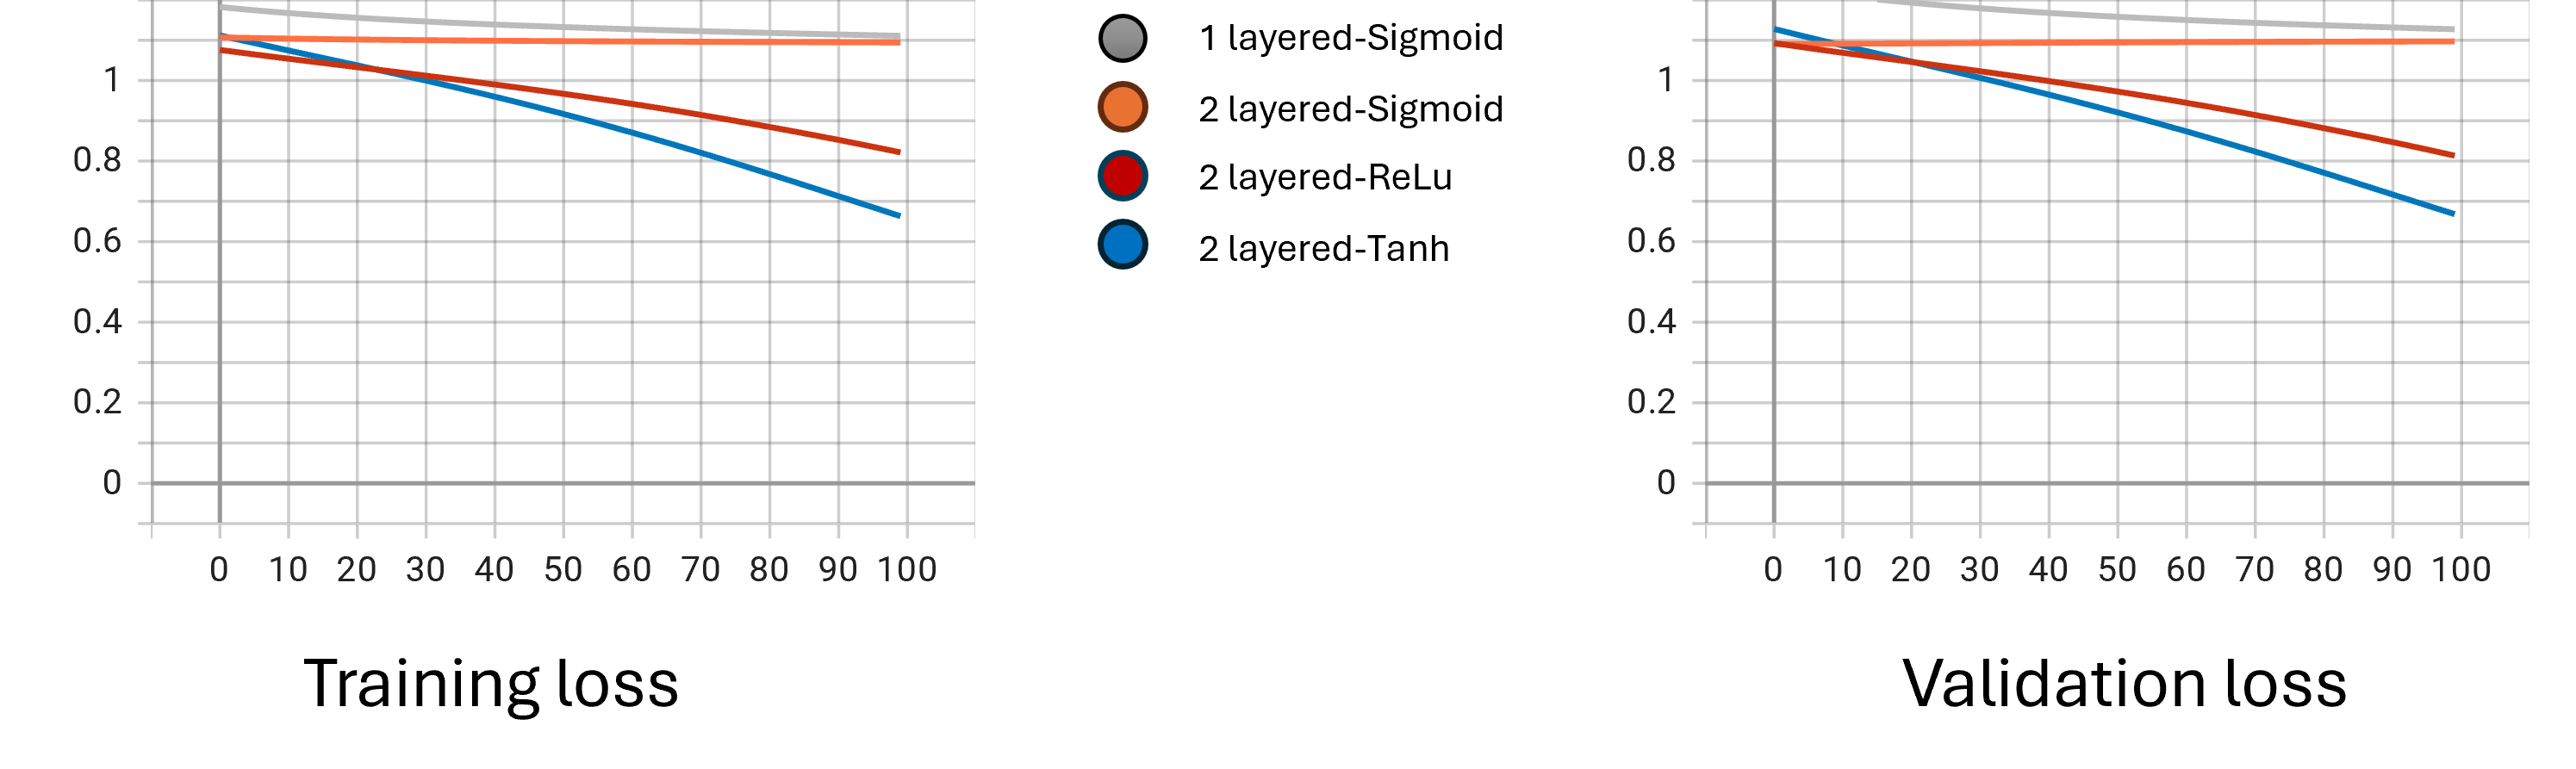
\includegraphics[width=1.0\textwidth]{./results/part_1/loss_sgd.png}
    \caption{loss SGD}
    \label{fig: loss curves-SGD}
\end{figure}

\begin{figure}
    \centering
    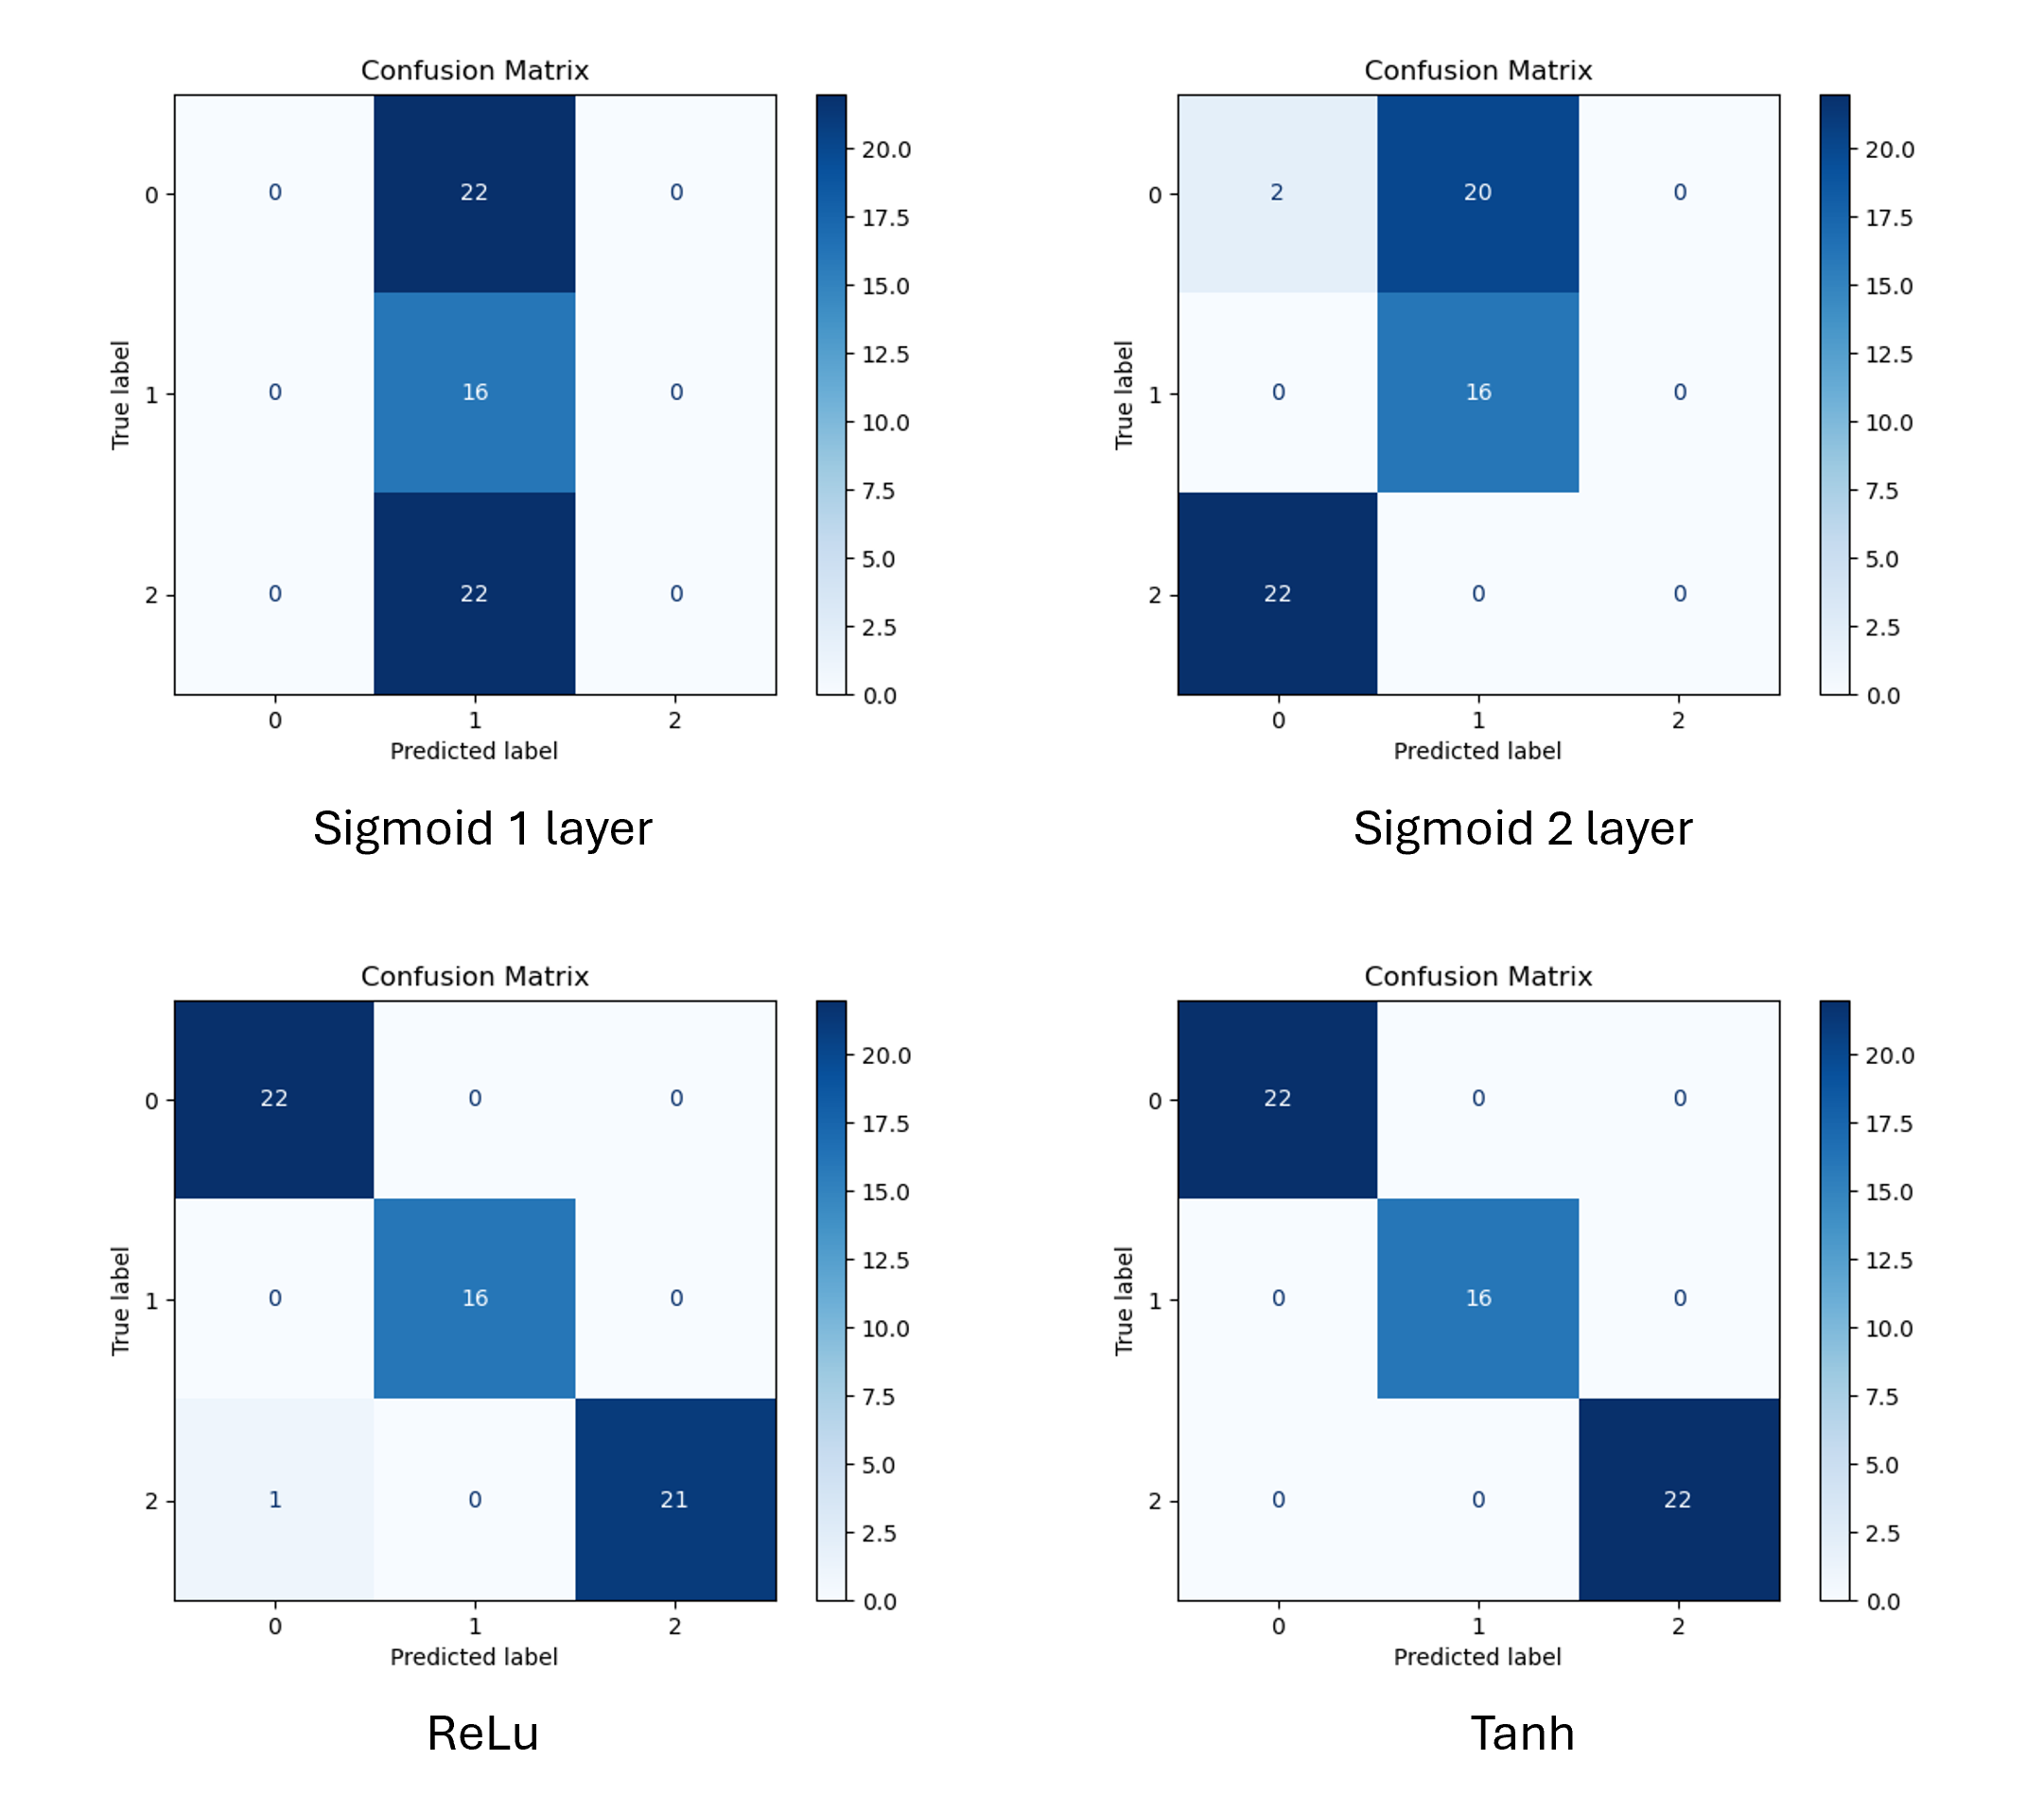
\includegraphics[width=0.8\textwidth]{./results/part_1/confustion_matrices/sgd.png}
    \caption{Confusion matrices for architectures optimized with \textbf{SGD}}
    \label{fig: cm SGD}
\end{figure}

\begin{figure}[t]
    \centering
    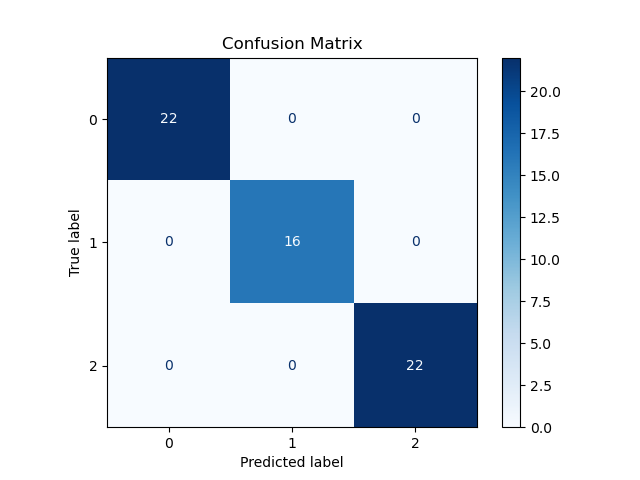
\includegraphics[width=0.5\textwidth]{./results/part_1/confustion_matrices/adam.png}
    \caption{Confusion matrix for all architectures optimized with \textbf{Adam}}
    \label{fig: cm adam}
\end{figure}


\subsection{Part 2}

\begin{figure}[h]
    \centering
    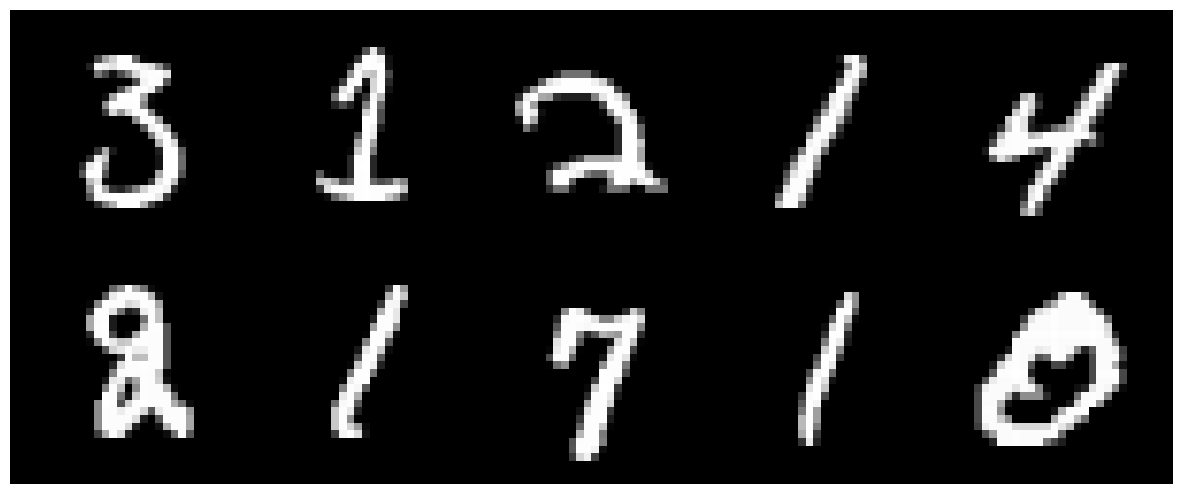
\includegraphics[width=0.5\textwidth]{./MNIST dataset.png}
    \caption{Samples from the MNIST dataset}
    \label{fig: mnsit}
\end{figure}

\subsubsection{Data}

The MNIST dataset (Samples of the dataset shown in figure \ref*{fig: mnsit}
was used in this part of the project to compare the efficacy (loosely defined)
and usefulness (loosely defined) of a CNN and an MLP. The Modified National Institute 
of Standards and Technology (MNIST) dataset is a widely used collection of 
70,000 handwritten digits, serving as a cornerstone for research in machine 
learning and image processing. Comprised of 60,000 training images and 10,000 
testing images, each labeled with its corresponding digit (0-9). 

\subsubsection{Model Architectures}

A \textbf{Convolutional Neural Network} and a 


\subsubsection{Results}

